% !TeX program = xelatex
% Báo cáo học phần Thực tập doanh nghiệp; bản mẫu gốc được giữ tại main.template.tex.
\documentclass[12pt,a4paper]{article}
\usepackage{fontspec}
\IfFontExistsTF{Times New Roman}{\setmainfont{Times New Roman}}{\setmainfont{TeX Gyre Termes}}
\IfFontExistsTF{Arial}{\setsansfont{Arial}}{\setsansfont{TeX Gyre Heros}}
\IfFontExistsTF{Courier New}{\setmonofont{Courier New}[Scale=0.85]}{\setmonofont{Latin Modern Mono}[Scale=0.85]}
\usepackage[a4paper,left=2.7cm,right=2.3cm,top=2.8cm,bottom=2.5cm,headheight=16pt]{geometry}
\usepackage{amsmath,amssymb,graphicx,booktabs,longtable,tabularx,array}
\usepackage[table]{xcolor}
\usepackage{tikz}
\usetikzlibrary{arrows.meta,positioning,calc,fit}
\usepackage{enumitem,caption,float,fancyhdr,titlesec,indentfirst}
\usepackage[hidelinks,unicode]{hyperref}
\definecolor{accent}{HTML}{246E85}
\definecolor{soft}{HTML}{EEF4F6}
\hypersetup{pdftitle={Trích xuất bảng từ văn bản bằng GLiNER2 và GPT 5.5},pdfauthor={Nguyễn Trần Huy},pdfsubject={Trích xuất cục bộ và hybrid - báo cáo Thực tập doanh nghiệp}}
\renewcommand{\contentsname}{Mục lục}
\renewcommand{\listfigurename}{Danh mục hình}
\renewcommand{\listtablename}{Danh mục bảng}
\renewcommand{\figurename}{Hình}
\renewcommand{\tablename}{Bảng}
\renewcommand{\refname}{Tài liệu tham khảo}
\renewcommand{\arraystretch}{1.25}
\setlength{\parskip}{4pt}
\setlength{\parindent}{1.2em}
\linespread{1.08}
\setlist{nosep,leftmargin=1.5em,topsep=5pt}
\captionsetup{font=small,labelfont=bf,skip=8pt}
\setlength{\emergencystretch}{2em}
\pagestyle{fancy}
\fancyhf{}
\fancyhead[L]{\footnotesize Trích xuất bảng bằng GLiNER2 và GPT 5.5}
\fancyhead[R]{\footnotesize UET - VNU}
\fancyfoot[C]{\thepage}
\renewcommand{\headrulewidth}{0.4pt}
\renewcommand{\footrulewidth}{0.4pt}
\titleformat{\section}{\normalfont\Large\bfseries}{\thesection}{.7em}{}
\titleformat{\subsection}{\normalfont\large\bfseries}{\thesubsection}{.7em}{}
\titleformat{\subsubsection}{\normalfont\normalsize\bfseries}{\thesubsubsection}{.7em}{}
\newcolumntype{Y}{>{\raggedright\arraybackslash}X}
\newcommand{\code}[1]{{\small\texttt{\detokenize{#1}}}}
\newcommand{\chapterstart}[1]{\clearpage\section{#1}}
\begin{document}
\pagenumbering{gobble}
\begin{titlepage}
\begin{tikzpicture}[overlay,remember picture]
\draw[line width=2pt] ($(current page.north west)+(2cm,-1.8cm)$) rectangle ($(current page.south east)+(-1.6cm,1.8cm)$);
\draw[line width=.7pt] ($(current page.north west)+(2.15cm,-1.95cm)$) rectangle ($(current page.south east)+(-1.75cm,1.95cm)$);
\end{tikzpicture}
\centering
{\fontsize{14}{17}\selectfont\bfseries ĐẠI HỌC QUỐC GIA HÀ NỘI}\\[.2cm]
{\fontsize{15}{18}\selectfont\bfseries TRƯỜNG ĐẠI HỌC CÔNG NGHỆ}\\[.2cm]
\rule{8cm}{.7pt}
\vspace{.65cm}


\includegraphics[width=2.9cm]{uet.png}
\vspace{.7cm}

{\fontsize{18}{22}\selectfont\bfseries BÁO CÁO HỌC PHẦN THỰC TẬP DOANH NGHIỆP}\\[.65cm]
{\fontsize{16}{20}\selectfont\bfseries ĐỀ TÀI}\\[.4cm]
{\fontsize{22}{27}\selectfont\bfseries TRÍCH XUẤT BẢNG TỪ VĂN BẢN\\[.15cm] BẰNG GLiNER2 VÀ GPT 5.5}\\[.45cm]
{\large Khảo sát phương pháp kết hợp trên dữ liệu RotoWire}
\vspace{1.1cm}

\begin{tabular}{@{}l l r@{}}
\textbf{Giảng viên hướng dẫn:}&ThS. Nguyễn Thị Thuỳ Linh&\\[.25cm]
\textbf{Sinh viên thực hiện:}&Nguyễn Trần Huy&23020378\\
\end{tabular}
\vfill
{\large\bfseries Hà Nội, tháng 9 năm 2026}
\end{titlepage}

\clearpage\thispagestyle{empty}
\begin{center}\Large\bfseries Ý KIẾN ĐÁNH GIÁ\end{center}
\vspace{.8cm}
\noindent\textbf{Ý kiến đánh giá:}\\[.5cm]
\foreach \n in {1,...,10}{\noindent\makebox[\textwidth]{\dotfill}\\[.6cm]}
\vspace{.5cm}
\noindent\textbf{Điểm số:} \dotfill\hspace{1cm}\textbf{Điểm chữ:}\dotfill
\vspace{1.3cm}
\begin{flushright}Hà Nội, ngày \dots, tháng \dots, năm 20\dots\\[1cm]
\textbf{Giảng viên đánh giá}\\\textit{(Ký, ghi rõ họ tên)}\end{flushright}

\clearpage\thispagestyle{empty}
\begin{center}\Large\bfseries LỜI CẢM ƠN\end{center}
\vspace{.6cm}
Em xin trân trọng cảm ơn cô ThS. Nguyễn Thị Thuỳ Linh đã cung cấp đề tài, hướng dẫn và hỗ trợ em trong quá trình thực hiện học phần Thực tập doanh nghiệp. Báo cáo này trình bày việc xây dựng và đánh giá hệ thống trích xuất bảng từ văn bản bằng GLiNER2 và GPT 5.5, với trọng tâm là trích xuất cục bộ, cơ chế hoạt động của mô hình và đánh giá trên dữ liệu thực tế.

Thông qua đề tài, em có cơ hội tìm hiểu cách tổ chức dữ liệu phi cấu trúc thành bảng, ứng dụng mô hình trích xuất trên máy tính cá nhân và kết hợp mô hình ngôn ngữ để đề xuất schema theo nội dung. Em hướng tới một giải pháp giảm phụ thuộc vào dịch vụ suy luận bên ngoài, đồng thời có cấu trúc linh hoạt để mở rộng cho nhiều loại văn bản.

Em kính mong nhận được góp ý để hoàn thiện phương pháp đánh giá, cách diễn giải kết quả và hướng phát triển của hệ thống.
\begin{flushright}Sinh viên thực hiện\\Nguyễn Trần Huy\end{flushright}

\clearpage
\pagenumbering{roman}
\section*{Tóm tắt}\addcontentsline{toc}{section}{Tóm tắt}
Dự án nghiên cứu phương pháp chuyển văn bản thành bảng bằng GLiNER2, với định hướng thực hiện phần trích xuất trên máy cục bộ. Khi schema được cung cấp sẵn và mô hình đã được tải, GLiNER2 có thể xử lý văn bản trên CPU mà không cần gửi nội dung tài liệu tới dịch vụ LLM. Cách triển khai này loại bỏ nhu cầu sử dụng token dịch vụ LLM cho bước trích xuất và giúp tổ chức giữ dữ liệu nội bộ trong môi trường do mình quản lý.

Để hỗ trợ văn bản có cấu trúc thông tin khác nhau, hệ thống còn có phương án hybrid: GPT 5.5 đề xuất schema từ một đoạn ngắn, còn GLiNER2 đọc toàn văn và điền các bản ghi cục bộ. Schema được xác định theo nội dung thay vì cố định một danh sách cột duy nhất. Phương án này giảm lượng văn bản cần gửi cho GPT, nhưng đoạn trích vẫn được xử lý bởi dịch vụ bên ngoài; không có số đo token hoặc chi phí tiền trong thực nghiệm.

Đánh giá sử dụng RotoWire, gồm báo cáo bóng rổ tiếng Anh và bảng tham chiếu. Trong điều kiện oracle schema tham chiếu, GLiNER2 đạt fact micro F1 44,53\% trên 200 mẫu test, với độ trễ trung bình 3,620 giây/bài; GPT nhận cùng schema đạt F1 68,68\%. Hybrid đạt precision 46,03\%, recall 17,59\% và F1 25,46\% trên 200 mẫu test; F1 của GPT trực tiếp trên cùng 200 mẫu là 9,27\% theo bộ chấm cố định. Độ trễ hybrid trung bình là 12,020 giây/bài. Kết quả xác nhận khả năng trích xuất cục bộ và cho thấy tiềm năng của cách kết hợp schema động; hiệu quả trên các miền văn bản khác cần được đánh giá riêng.

\noindent\textbf{Từ khóa:} GLiNER2, trích xuất thông tin, xử lý cục bộ, schema động, hybrid, RotoWire.
\clearpage\setcounter{tocdepth}{2}\tableofcontents
\clearpage\listoffigures\listoftables
\clearpage\pagenumbering{arabic}
\section{Giới thiệu về tập dữ liệu}
\subsection{Động lực: trích xuất cục bộ và sử dụng dữ liệu nội bộ}
Trong nhiều tổ chức, thông tin phục vụ công việc được lưu dưới dạng báo cáo, hồ sơ, mô tả sản phẩm hoặc thư trao đổi. Để tìm kiếm, tổng hợp và phân tích, các tài liệu này cần được chuyển thành bản ghi có cấu trúc. Nếu giao toàn bộ việc đọc và tạo bảng cho một LLM chạy trên dịch vụ bên ngoài, nội dung văn bản phải được truyền tới dịch vụ đó và việc xử lý phụ thuộc vào tài nguyên suy luận của nhà cung cấp.

Dự án lựa chọn GLiNER2 để thực hiện phần trích xuất ngay trên máy tính của người dùng. Với trọng số đã được tải và schema được cung cấp, mô hình chạy bằng CPU cục bộ; văn bản và bảng kết quả có thể được giữ trong môi trường nội bộ. Trong cấu hình này, bước trích xuất không cần gọi một dịch vụ LLM, nhờ đó không phát sinh token dịch vụ LLM cho từng tài liệu. GLiNER2 vẫn có quá trình token hóa và sử dụng tài nguyên tính toán tại máy; lợi ích được nhấn mạnh là giảm phụ thuộc vào suy luận thuê ngoài.

Khả năng chạy cục bộ tạo điều kiện kiểm soát dữ liệu tốt hơn: tổ chức không cần gửi nội dung tài liệu cho bên thứ ba để điền các trường đã xác định. Tổ chức có thể chủ động lựa chọn nơi lưu văn bản, nơi lưu kết quả và quyền truy cập trong môi trường triển khai của mình.

Một yêu cầu khác là hỗ trợ nhiều loại văn bản có các trường thông tin khác nhau. Dự án sử dụng thêm phương án hybrid: GPT đề xuất schema theo nội dung đoạn trích, sau đó GLiNER2 áp dụng schema đó lên toàn bài. Ví dụ, cùng luồng xử lý có thể được thiết kế để nhận các trường của báo cáo thể thao, mô tả sản phẩm hoặc hồ sơ nhân sự. Các ví dụ này minh họa khả năng mở rộng của thiết kế; thực nghiệm trong báo cáo mới kiểm chứng trên văn bản bóng rổ tiếng Anh.

\subsection{Hai chế độ sử dụng và phạm vi dữ liệu gửi đi}
\begin{table}[H]
\centering\small
\begin{tabularx}{\linewidth}{@{}p{3.15cm}Y Y@{}}
\toprule
\textbf{Tiêu chí} & \textbf{GLiNER2 local} & \textbf{Hybrid GPT + GLiNER2}\\\midrule
Nguồn schema & Người dùng hoặc ứng dụng cung cấp. & GPT đề xuất từ đoạn văn bản ngắn.\\
Phần điền dữ kiện & GLiNER2 xử lý toàn văn trên máy. & GLiNER2 xử lý toàn văn trên máy.\\
Văn bản gửi dịch vụ LLM & Không cần gửi để suy luận. & Có gửi đoạn trích cho GPT.\\
Sử dụng token dịch vụ LLM & Không cần cho bước trích xuất. & Cần cho yêu cầu tạo schema; không dùng GPT để điền toàn bảng.\\
Tình huống phù hợp về thiết kế & Bộ trường đã biết; ưu tiên giữ tài liệu tại chỗ. & Loại thông tin thay đổi; cần đề xuất bộ trường theo nội dung.\\
\bottomrule
\end{tabularx}
\caption{Hai chế độ xử lý và ranh giới dữ liệu. Lợi ích về token là phân tích thiết kế, chưa được đo định lượng.}
\label{tab:modes}
\end{table}

Hybrid chỉ gửi một đoạn giữa nguyên văn, tối đa 10\% số từ và không quá 80 từ của bài. Cách phân công này làm giảm lượng nội dung văn bản gửi tới GPT so với yêu cầu GPT đọc toàn bài. Tuy nhiên, số từ không bằng số token và yêu cầu còn chứa lời nhắc cùng mô tả định dạng; báo cáo không suy ra một tỷ lệ tiết kiệm token hoặc tiền cụ thể. Đoạn trích cũng có thể chứa dữ liệu nhạy cảm, nên hybrid không có cùng mức giữ kín nội dung như cấu hình hoàn toàn cục bộ.

\subsection{Bài toán text-to-table và nguồn RotoWire}
Text-to-table là bài toán tạo một hoặc nhiều bảng thể hiện nội dung của văn bản, bao gồm xác định trường và điền thông tin tương ứng \cite{t2t}. Trong dự án, đầu vào là văn bản tiếng Anh và đầu ra là bảng dữ liệu, chưa bao gồm bước sinh truy vấn SQL. Để đánh giá khả năng trích xuất, mỗi dự đoán được đối chiếu với bảng tham chiếu, còn gọi là gold.

RotoWire được chọn vì các bài tường thuật bóng rổ chứa nhiều đối tượng và thống kê đan xen: tên cầu thủ, tên đội, điểm số, rebounds, assists, thành tích ném và tỷ số trận. Đây là điều kiện phù hợp để kiểm tra không chỉ việc tìm con số mà còn việc gắn con số vào đúng người, đúng thuộc tính và đúng phạm vi thời gian.

Dự án sử dụng bản chuyển thể thuộc nguồn \code{xqwu/text-to-table}, phần RotoWire. Văn bản và bảng tương ứng được đọc theo cặp, giữ nguyên liên kết giữa nội dung bài và nhãn tham chiếu. Phiên bản dữ liệu được cố định bằng revision và băm tệp để các phép so sánh dùng cùng đầu vào.

\subsection{Cấu trúc dữ liệu và ví dụ minh họa}
Bảng tham chiếu gồm hai nhóm chính. Bảng cầu thủ có mỗi hàng là một cầu thủ và các cột là thống kê của người đó. Bảng đội mô tả số liệu gắn với đội, có thể gồm điểm, thành tích hoặc thống kê theo phạm vi của trận. Tên hàng là định danh đối tượng; tên cột là thuộc tính cần trích xuất. Hai thành phần này có vai trò khác nhau.

Xét đoạn minh họa không thuộc các mẫu tính điểm:
\begin{quote}
Alex scored 24 points and grabbed seven rebounds. Ben added 18 points.
\end{quote}
Một bảng phù hợp với đoạn này có dạng:
\begin{table}[H]
\centering
\begin{tabular}{@{}lrr@{}}
\toprule\textbf{Cầu thủ} & \textbf{Points} & \textbf{Rebounds}\\\midrule
Alex & 24 & 7\\
Ben & 18 & Chưa có thông tin\\
\bottomrule
\end{tabular}
\caption{Ví dụ chuyển văn bản thành bảng; ô chưa có thông tin không được tự điền 0.}
\end{table}

Trong ví dụ, lấy được số 24 nhưng gắn vào Ben hoặc vào cột rebounds vẫn là sai dữ kiện. Thực tế RotoWire còn có các trường hợp khó hơn: tên người ở câu trước, số liệu ở câu sau; thống kê hiệp đầu cạnh tổng cả trận; thành tích của trận trước cạnh trận hiện tại; tổng điểm của nhiều người trong cùng một câu. Vì vậy, việc đánh giá cần xét đồng thời đối tượng, trường và giá trị.

\subsection{Phân chia dữ liệu sử dụng trong dự án}
\begin{table}[H]
\centering
\begin{tabularx}{\linewidth}{@{}Yrrr@{}}
\toprule\textbf{Hạng mục} & \textbf{Nguồn có sẵn} & \textbf{Số mẫu sử dụng} & \textbf{Seed}\\\midrule
Validation & 727 & 30 & 43\\
Test & 728 & 200 & 42\\
\bottomrule
\end{tabularx}
\caption{Quy mô dữ liệu được cố định trong manifest.}
\end{table}

Tổng số dữ kiện gold sau chuẩn hóa là 853 trên 30 mẫu validation và 6156 trên 200 mẫu test. Validation được dùng để lựa chọn cấu hình GLiNER2; sau đó cấu hình được giữ cố định khi chạy test. Tất cả kết quả chính trong báo cáo đều dùng cùng 200 mẫu test, gồm GLiNER2 local, GPT với schema cho trước, hybrid và GPT tạo bảng trực tiếp. Danh sách ID, nội dung văn bản và gold được đối chiếu để bảo đảm các phép so sánh dùng cùng dữ liệu.

Chương trình kiểm tra trùng văn bản nhưng chưa có khóa ghép đủ tin cậy để loại sạch các bài cùng trận giữa các phần dữ liệu. Gold và từ điển chuẩn hóa được giữ cố định khi tính điểm. Những yếu tố này được xét khi diễn giải kết quả, đặc biệt là khả năng áp dụng sang dữ liệu ngoài tập đánh giá.

\chapterstart{Kiến trúc và cách hoạt động GLiNER2}
\subsection{Tổng quan mô hình}
GLiNER2 là mô hình trích xuất thông tin theo schema, phát triển từ hướng tiếp cận dùng Transformer encoder. Công trình giới thiệu khả năng nhận diện thực thể, phân loại văn bản và trích xuất cấu trúc trong cùng một hệ thống \cite{gliner}. Dự án tập trung vào trích xuất cấu trúc: mỗi loại đối tượng có nhiều bản ghi, mỗi bản ghi gồm định danh và các thuộc tính.

Checkpoint được sử dụng là \code{fastino/gliner2-base-v1}. Cấu hình trọng số cục bộ chỉ định backbone \code{microsoft/deberta-v3-base}, cơ chế biểu diễn các đoạn văn bản có độ rộng tối đa tám từ theo bộ xử lý, và lớp tạo biểu diễn bản ghi \code{count_lstm_v2}. Thư viện đang dùng là GLiNER2 1.2.4. Các mô tả kỹ thuật dưới đây được đối chiếu trực tiếp với cấu hình và mã thư viện dùng trong dự án, không lấy thông số của phiên bản khác để thay thế.

Một đặc điểm quan trọng là schema cũng là đầu vào của mô hình. Khi thay tên trường và mô tả, mô hình nhận một yêu cầu trích xuất khác mà không bắt buộc thay kiến trúc mạng. Chính đặc điểm này tạo cơ sở cho hai chế độ: nhận schema từ ứng dụng hoặc nhận schema do GPT đề xuất.

\subsection{Mã hóa đồng thời schema và văn bản}
Schema khai báo loại bản ghi và các thuộc tính cần lấy. Ví dụ, với bài tường thuật bóng rổ, cấu trúc có thể là \textit{player}, gồm \textit{name}, \textit{points} và \textit{rebounds}. Bộ xử lý biến cấu trúc này thành chuỗi có các ký hiệu phân biệt thành phần schema, rồi đặt cùng văn bản để đưa vào encoder. Dạng khái quát là
\begin{equation}
X = \operatorname{serialize}(S)\oplus[\mathrm{SEP}]\oplus D,
\end{equation}
trong đó $S$ là schema, $D$ là văn bản và $\oplus$ là phép ghép chuỗi đầu vào.

Encoder tạo các vector ngữ cảnh cho cả tên trường và các từ của văn bản. Nhờ đọc cùng nhau, biểu diễn của một trường như \textit{points} có thể được xét trong ngữ cảnh thống kê cầu thủ, còn các cụm số trong văn bản được biểu diễn với thông tin xung quanh. Chương trình giữ tên trường có nghĩa và mô tả ngắn về nội dung, kiểu giá trị và đơn vị để yêu cầu trích xuất được thể hiện rõ.

Việc dùng encoder có nghĩa mô hình tính biểu diễn của đầu vào trước khi chấm điểm các đoạn ứng viên. Ở đường trích xuất đang sử dụng, GLiNER2 chọn các đoạn của văn bản rồi phần mềm tổ chức chúng thành cấu trúc đầu ra; mô hình không cần sinh toàn bộ bảng bằng một chuỗi token văn bản tự hồi quy như cách một LLM tạo JSON.

\begin{figure}[H]
\centering
\begin{tikzpicture}[node distance=7mm and 9mm, box/.style={draw=accent,rounded corners,fill=soft,align=center,text width=5.55cm,minimum height=13mm,font=\small},wide/.style={box,text width=12.1cm},arr/.style={-{Latex},thick,draw=accent}]
\node[wide] (input) {Schema có tên trường và mô tả + văn bản đầu vào};
\node[wide,below=of input] (encoder) {Tokenizer và Transformer encoder DeBERTa-v3-base\\Tạo biểu diễn ngữ cảnh cho schema và văn bản};
\node[box,below left=8mm and -5.55cm of encoder] (span) {Nhánh văn bản\\Biểu diễn các đoạn ứng viên};
\node[box,right=of span] (count) {Nhánh schema\\Dự đoán số bản ghi $K$};
\node[box,below=of count] (instance) {Tạo biểu diễn riêng\\cho mỗi cặp bản ghi--thuộc tính};
\node[wide,below=23mm of span,xshift=3.275cm] (score) {Chấm điểm tương thích đoạn--thuộc tính--bản ghi\\Sigmoid, ngưỡng chọn và giải mã};
\node[wide,below=of score] (output) {Các bản ghi có cấu trúc\\Định danh và giá trị trích từ văn bản};
\draw[arr](input)--(encoder);\draw[arr](encoder.south)-|(span.north);\draw[arr](encoder.south)-|(count.north);\draw[arr](count)--(instance);\draw[arr](span.south)--(score.north -| span.south);\draw[arr](instance.south)--(score.north -| instance.south);\draw[arr](score)--(output);
\end{tikzpicture}
\caption{Các thành phần suy luận của GLiNER2 cho trích xuất cấu trúc, giản lược từ mã thư viện dùng trong dự án.}
\label{fig:model}
\end{figure}

\subsection{Biểu diễn các đoạn giá trị trong văn bản}
Một đoạn liên tiếp của văn bản, gọi là \textit{span}, có thể là tên người, tên đội, một con số hoặc một cụm giá trị. Từ biểu diễn ngữ cảnh, lớp span tạo vector cho các cặp vị trí bắt đầu và kết thúc hợp lệ. Trong checkpoint đang dùng, chương trình xét các đoạn có độ rộng không quá tám từ theo cách tách từ của bộ xử lý.

Với ví dụ ``Alex scored 24 points'', các ứng viên bao gồm tên Alex, số 24 và các cụm liên tiếp khác. Mục tiêu không phải lấy mọi ứng viên mà chấm mức phù hợp của từng ứng viên với thuộc tính đang xét. Cùng một số 24 có thể đạt điểm cao cho trường points nhưng không phù hợp với trường định danh.

Giới hạn độ rộng span và giới hạn chiều dài đầu vào giúp giới hạn lượng tính toán, đồng thời tạo ràng buộc đối với văn bản dài hoặc giá trị kéo dài. Ở cấp chương trình, toàn bài được chia thành các cửa sổ phù hợp rồi ghép kết quả, thay vì coi một lần gọi mô hình là đã bao phủ mọi văn bản.

\subsection{Dự đoán số bản ghi và phân biệt các đối tượng}
Một schema có thể tương ứng với nhiều đối tượng trong cùng văn bản. Nếu chỉ tìm mọi tên người và mọi con số một cách độc lập, hệ thống chưa biết ghép giá trị nào cho hàng nào. Đường trích xuất cấu trúc của GLiNER2 sử dụng một bước dự đoán số bản ghi và biểu diễn thuộc tính riêng cho từng bản ghi để giải quyết nhiệm vụ này.

Cụ thể, vector đại diện cấu trúc được đưa qua một mạng MLP để tạo điểm cho số lượng bản ghi. Mã thư viện có 20 lớp, tương ứng số lượng từ 0 đến 19; lúc suy luận, chương trình lấy lớp có điểm lớn nhất:
\begin{equation}
\widehat K=\underset{k\in\{0,\ldots,19\}}{\operatorname{argmax}}\;c_k.
\end{equation}
Đây là dự đoán của mô hình trong một đơn vị xử lý, không phải số hàng lấy từ bảng gold. Tài liệu dài có thể được xử lý qua nhiều cửa sổ nên giới hạn này không phải giới hạn cố định 19 hàng cho toàn bộ tài liệu sau khi ghép.

Sau đó, mô-đun \code{count_lstm_v2} tạo các vector thuộc tính có điều kiện theo vị trí bản ghi. Trong bản mã thực tế, thành phần này dùng embedding vị trí đã học và GRU, mặc dù tên lớp có chữ LSTM. Với $m$ thuộc tính và $\widehat K$ bản ghi, đầu ra cung cấp biểu diễn cho $\widehat K\times m$ cặp bản ghi--thuộc tính.

Nhờ đó, trường points của bản ghi thứ nhất và trường points của bản ghi thứ hai có hai vector riêng để đối chiếu với văn bản. Trong ví dụ Alex và Ben, mô hình có thể lựa chọn giá trị 24 cho một hàng và 18 cho hàng còn lại. Cơ chế này hỗ trợ liên kết cấu trúc, nhưng việc gắn đúng ngữ nghĩa vẫn cần được kiểm chứng bằng kết quả thực nghiệm.

\subsection{Chấm điểm và dựng cấu trúc đầu ra}
Gọi $v_{ij}$ là vector của đoạn từ vị trí $i$ đến $j$, và $u_{km}$ là vector thuộc tính $m$ ở bản ghi $k$. Phép tính trong đường suy luận có thể viết gọn thành
\begin{equation}
p_{k,m,i,j}=\sigma\!\left(v_{ij}^{\mathsf T}u_{km}\right),
\end{equation}
trong đó $\sigma$ là hàm sigmoid. Điểm này được dùng cùng ngưỡng và quy tắc giải mã để lấy các đoạn tương ứng. Không diễn giải trực tiếp điểm sigmoid như một xác suất đúng đã được hiệu chỉnh cho dữ liệu RotoWire.

Trong cấu hình dự án, ngưỡng là 0,5. Khóa định danh được khai báo kiểu chuỗi, còn thuộc tính có thể giữ danh sách giá trị. Cách lưu danh sách bảo toàn những trường hợp có nhiều giá trị trích được; bước ghép không chọn một giá trị chỉ vì nó giống gold. Dữ kiện được chuẩn hóa thành bộ gồm loại bảng, đối tượng, trường và giá trị để chấm sau suy luận.

Mô hình lấy các đoạn xuất hiện trong văn bản không đồng nghĩa mọi ô đều đúng. Một số có thể thuộc cầu thủ khác, thuộc trận trước hoặc chỉ là thống kê một hiệp. Vì vậy, đánh giá cuối xét cả định danh và phạm vi trường, không chỉ kiểm tra con số có xuất hiện trong bài hay không.

\subsection{Cách sử dụng GLiNER2 trong chương trình}
Toàn bộ trọng số GLiNER2 được nạp một lần vào CPU và sử dụng lại cho các tài liệu. Cấu hình cuối giữ tên trường có nghĩa, mô tả gọn và thực hiện riêng từng bảng. Khi trích bảng cầu thủ, mô hình nhận schema cầu thủ cùng toàn văn; khi trích bảng đội, mô hình nhận schema đội cùng toàn văn.

Ngân sách đầu vào gồm cả schema và văn bản. Giới hạn vận hành đã kiểm tra trong checkpoint dùng cho dự án là 512 token nội bộ. Adapter chọn các cửa sổ vừa giới hạn, ưu tiên biên câu khi có thể và giữ phần chồng lấn để giảm mất ngữ cảnh ở biên. Mọi cửa sổ cần thiết đều được chạy; thời gian ghi nhận gồm tổng xử lý các bảng và các đoạn.

Kết quả từ nhiều cửa sổ được ghép theo định danh chuẩn hóa. Giá trị trùng được loại lặp; giá trị khác nhau vẫn được giữ như xung đột cần chấm hoặc xem lại. Sau khi nạp trọng số, các bước này đều thực hiện tại máy, phù hợp với mục tiêu xử lý dữ liệu nội bộ mà không gọi LLM để điền từng ô.

\subsection{Kết hợp GPT để đề xuất schema động}
\subsubsection{Vai trò của GPT}
Khi loại văn bản thay đổi, bộ trường hữu ích cũng thay đổi. Hybrid dùng GPT cho bước đọc hiểu đoạn trích và đề xuất schema, còn GLiNER2 đảm nhiệm phần trích xuất dữ kiện. GPT chỉ trả tên bảng, tên thuộc tính, mô tả, kiểu giá trị và đơn vị nếu có căn cứ; không đưa tên đối tượng cụ thể hoặc giá trị quan sát được vào schema.

Lời nhắc yêu cầu chỉ đề xuất trường có bằng chứng trong đoạn nhận được, phân biệt định danh với thuộc tính và giữ phạm vi của thống kê. Nếu đoạn không có đủ thông tin, schema rỗng được chấp nhận. Chương trình không tự bổ sung bộ cột phổ biến từ gold và không gửi toàn bài cho GPT để sửa đầu ra trong cấu hình hybrid này.

\subsubsection{Chọn đoạn và luồng xử lý}
Với $N$ từ được tách theo khoảng trắng, chương trình chọn
\begin{equation}
B=\min\left(80,\left\lfloor\frac{N}{10}\right\rfloor\right)
\end{equation}
từ liên tục ở giữa bài. Chỉ đoạn này được đưa vào phần dữ liệu văn bản của yêu cầu GPT; GLiNER2 vẫn đọc toàn bài. Lời nhắc và khung định dạng là phần riêng, không nằm trong tỷ lệ số từ nêu trên.

\begin{figure}[H]
\centering
\begin{tikzpicture}[node distance=8mm and 10mm,box/.style={draw=accent,rounded corners,fill=soft,align=center,text width=5.5cm,minimum height=13mm,font=\small},arr/.style={-{Latex},thick,draw=accent}]
\node[box] (full) {Toàn văn trên máy cục bộ};
\node[box,right=of full,fill=white] (snippet) {Đoạn giữa tối đa 10\% số từ\\và không quá 80 từ};
\node[box,below=of snippet,fill=white] (gpt) {Dịch vụ GPT 5.5\\Đề xuất schema từ đoạn trích};
\node[box,below=of gpt] (schema) {Schema trả về máy\\Kiểm tra cấu trúc và thuộc tính};
\node[box,left=of schema] (gliner) {GLiNER2 cục bộ\\Áp dụng schema lên toàn văn};
\node[box,below=of gliner] (table) {Bảng kết quả trên máy};
\draw[arr](full)--(snippet);\draw[arr](snippet)--(gpt);\draw[arr](gpt)--(schema);\draw[arr](schema)--(gliner);\draw[arr](full)--(gliner);\draw[arr](gliner)--(table);
\end{tikzpicture}
\caption{Luồng hybrid và ranh giới xử lý: đoạn trích được gửi tới GPT; toàn văn dùng cho GLiNER2 được xử lý cục bộ.}
\label{fig:hybrid}
\end{figure}

Thiết kế chuyển phần tạo schema cho GPT giúp chương trình không bị buộc vào một danh mục cột duy nhất. Tuy vậy, chất lượng schema phụ thuộc thông tin có trong đoạn trích. Nếu trường cần thiết chưa được đề xuất, GLiNER2 không tự thêm trường đó trong giao thức hiện tại.

\subsubsection{Khả năng mở rộng cho nhiều loại văn bản}
Tầng mô hình trích xuất nhận schema làm đầu vào nên có thể tái sử dụng cùng cách gọi cho các loại bản ghi khác nhau. Bảng~\ref{tab:domains} minh họa cách thay schema khi thay loại tài liệu; các ví dụ không phải kết quả benchmark của dự án.

\begin{table}[H]
\centering\small
\begin{tabularx}{\linewidth}{@{}p{3.2cm}p{2.5cm}Y@{}}
\toprule\textbf{Loại văn bản} & \textbf{Loại bản ghi} & \textbf{Thuộc tính có thể cần trích}\\\midrule
Báo cáo thể thao & Cầu thủ, đội & Points, rebounds, assists, thống kê đội.\\
Mô tả sản phẩm & Sản phẩm & Tên, giá, nhãn hiệu, thông số được nêu.\\
Hồ sơ nhân sự & Ứng viên & Tên, kỹ năng, kinh nghiệm, học vấn.\\
Báo cáo doanh nghiệp & Tổ chức & Tên, chỉ tiêu được công bố, kỳ báo cáo.\\
\bottomrule
\end{tabularx}
\caption{Ví dụ định hướng mở rộng bằng schema; mới có miền bóng rổ được đánh giá trong báo cáo.}
\label{tab:domains}
\end{table}

Khi chuyển miền, phần chuẩn bị dữ liệu, lời nhắc, mô tả schema và tiêu chí chấm cũng cần được điều chỉnh. Bộ benchmark hiện có nhiều quy tắc dành cho RotoWire; chưa phải một ứng dụng đa miền đã được xác nhận độ chính xác. Lợi ích của hybrid ở đây là cấu trúc xử lý linh hoạt để phát triển theo hướng đó, trong khi phần điền dữ liệu tiếp tục dùng mô hình cục bộ.

\chapterstart{Kết quả thí nghiệm và so sánh}
\subsection{Mục tiêu và thiết kế đánh giá}
Thực nghiệm tập trung vào hai câu hỏi. Thứ nhất, GLiNER2 có thể trích xuất bảng trên máy cục bộ với chất lượng và thời gian như thế nào khi được cung cấp schema? Thứ hai, khi schema được GPT đề xuất từ một đoạn ngắn, phương án hybrid cho kết quả ra sao so với GPT đọc toàn bài và tạo bảng trực tiếp?

Báo cáo trình bày cấu hình GLiNER2 cuối đã chọn trên validation và đánh giá trên 200 mẫu test. Các phương pháp dùng cùng văn bản và gold, nhưng được chia thành hai điều kiện: schema tham chiếu và tự xác định schema. Đối chiếu GLiNER2 local với GPT trong điều kiện schema tham chiếu đánh giá việc điền dữ kiện; đối chiếu hybrid với GPT trực tiếp đánh giá toàn bộ quá trình từ xác định trường đến tạo bảng. Không quy chênh lệch giữa hai điều kiện chỉ cho năng lực mô hình, vì lượng thông tin đầu vào khác nhau.

\begin{table}[H]
\centering\small
\begin{tabularx}{\linewidth}{@{}p{3.3cm}p{2.1cm}Y@{}}
\toprule\textbf{Phương pháp} & \textbf{Tập đánh giá} & \textbf{Thông tin được cung cấp}\\\midrule
GLiNER2 local & 200 test & Toàn văn và tên bảng/cột từ schema tham chiếu của từng bài; không có tên hàng hoặc giá trị gold.\\
GPT schema tham chiếu & Cùng 200 test & Toàn văn và cùng tên bảng/cột tham chiếu như GLiNER2 local.\\
Hybrid & 200 test & GPT nhận đoạn giữa để đề xuất schema; GLiNER2 nhận schema và toàn văn.\\
GPT trực tiếp & Cùng 200 test & Toàn văn; tự xác định trường và tạo bảng.\\
\bottomrule
\end{tabularx}
\caption{Các phương pháp được báo cáo và điều kiện đầu vào.}
\end{table}

Schema trong hai dòng đầu được dựng từ tên bảng và cột trong gold của chính từng tài liệu. Đây là điều kiện oracle nhằm cô lập bước trích xuất dữ kiện: mô hình không nhận tên hàng hay giá trị gold, nhưng schema không phải thứ hệ thống phải tự suy ra trước khi đọc bài. Vì vậy, kết quả của hai dòng này không đại diện trực tiếp cho một triển khai mà schema chưa được cấu hình từ bên ngoài.

Hai chế độ GPT và hybrid sử dụng kết quả đã lưu; GLiNER2 local được chạy với cấu hình cố định trên đúng 200 ID này. Các đầu ra được chấm theo cùng quy tắc. Các lượt đo diễn ra ở thời điểm khác nhau, nên so sánh dùng cho chất lượng; độ trễ mô tả từng lượt, không dùng để kết luận một tỷ lệ tăng tốc giữa các chiến dịch.

\subsection{Môi trường và cấu hình}
Máy thực nghiệm dùng Apple M1, RAM 16 GiB, macOS ARM64 và Python 3.11.14. GLiNER2 chạy trên CPU, float32, bốn luồng, batch size 1; không yêu cầu GPU trong các phép đo được trình bày. Checkpoint là \code{fastino/gliner2-base-v1}, với revision được cố định:
\begin{center}\code{8437ba583a733d87f56ae902f3b197934eedd58e}\end{center}
 Trọng số không được huấn luyện lại trong dự án.

Schema GLiNER2 giữ tên trường có nghĩa và mô tả gọn; mỗi bảng được thực thi riêng trên toàn bài qua các cửa sổ cần thiết. Ngưỡng trích xuất là 0,5. GPT dùng \code{gpt-5.5}, mức suy luận low, qua Codex CLI 0.154.0-alpha.6.2 và tài khoản ChatGPT; mỗi tác vụ là một phiên mới. Nhánh hybrid không dùng GPT để điền giá trị cuối cùng.

Dữ liệu, schema theo chế độ, lời nhắc và quy tắc chấm được cố định trong từng chiến dịch. Gold chỉ được dùng khi chấm; ở chế độ biết trước schema, mô hình được cung cấp tên bảng/cột nhưng không nhận dữ liệu trong các ô tham chiếu.

\subsection{Chỉ số đánh giá}
\subsubsection{Độ chính xác dữ kiện}
Một dữ kiện là bộ bốn gồm loại bảng, đối tượng, trường và giá trị. Dự đoán chỉ khớp khi các thành phần tương ứng khớp sau chuẩn hóa. Ví dụ, số điểm đúng nhưng gắn nhầm cầu thủ vẫn bị tính là một dữ kiện dự đoán sai và một dữ kiện gold bị thiếu.

Từ tập dự đoán $P_d$ và gold $G_d$ của mỗi tài liệu, chương trình cộng số khớp đúng $TP$, số dự đoán thừa hoặc sai $FP$ và số bị bỏ sót $FN$ trên toàn bộ mẫu. Các chỉ số chính là
\begin{equation}
\mathrm{Precision}=\frac{TP}{TP+FP},\quad
\mathrm{Recall}=\frac{TP}{TP+FN},\quad
F_1=\frac{2TP}{2TP+FP+FN}.
\end{equation}
Đây là fact micro F1, không phải tỷ lệ tài liệu hoàn toàn đúng. Dữ kiện trùng không được tính thêm điểm; null khác 0; các trường lạ vẫn nằm trong dự đoán. Tên bảng, trường và giá trị được chuẩn hóa bằng quy tắc cố định cho các phương pháp.

Mọi mẫu đã thử đều nằm trong điểm tổng, kể cả đầu ra rỗng hoặc lỗi thực thi. Kết quả hợp lệ về cấu trúc chỉ xác nhận chương trình có thể đọc và kiểm tra đầu ra, không xác nhận dữ kiện đúng. Ngoài F1, báo cáo dùng độ bao phủ schema để xác định phần dữ kiện gold thuộc các trường được GPT đề xuất.

\subsubsection{Thời gian và phạm vi đo token}
Độ trễ toàn tác vụ được đo từ lúc chuẩn bị đầu vào đến lúc có bảng cuối hoặc trạng thái lỗi. Với hybrid, thời gian bao gồm GPT tạo schema, GLiNER2 xử lý toàn văn, ghép kết quả và hậu xử lý. Tải trọng số, làm nóng mô hình, chấm điểm và dựng báo cáo không nằm trong thời gian xử lý từng bài.

Thực nghiệm không thống kê token hoặc quy đổi tiền. Vì vậy, nhận định về tiết kiệm token được giới hạn ở thiết kế: GLiNER2 local không gọi dịch vụ LLM để trích xuất; hybrid thu hẹp phần văn bản gửi GPT và chỉ yêu cầu schema thay vì bảng dữ liệu đầy đủ. Chưa có tỷ lệ tiết kiệm token hay chi phí được xác nhận bằng số đo.

\subsection{So sánh trong điều kiện schema tham chiếu trên 200 mẫu test}
Cấu hình GLiNER2 local được giữ nguyên sau khi chọn trên validation và hoàn tất 200/200 mẫu test, với 200/200 đầu ra hợp lệ. Với 6156 dữ kiện gold, mô hình trích khớp 2551 dữ kiện, tạo 2751 dự đoán thừa hoặc sai và bỏ sót 3605 dữ kiện. GLiNER2 và GPT đều nhận cùng tên bảng/trường lấy từ gold của từng bài, nhưng không nhận tên hàng hoặc giá trị gold.

\begin{table}[H]
\centering
\begin{tabularx}{\linewidth}{@{}Yrr@{}}
\toprule
\textbf{Chỉ số} & \textbf{GLiNER2 local} & \textbf{GPT schema tham chiếu} \\\midrule
Precision & 48,11\% & 72,16\% \\
Recall & 41,44\% & 65,51\% \\
Fact micro F1 & \textbf{44,53\%} & \textbf{68,68\%} \\
TP / FP / FN & 2551 / 2751 / 3605 & 4033 / 1556 / 2123 \\
Đầu ra hợp lệ & 200/200 & 200/200 \\
\bottomrule
\end{tabularx}

\caption{So sánh GLiNER2 local và GPT trong điều kiện oracle schema tham chiếu trên cùng 200 mẫu test.}
\label{tab:local}
\end{table}

GLiNER2 local đạt F1 44,53\%, thấp hơn 24,15 điểm phần trăm so với GPT trong điều kiện schema tham chiếu (68,68\%). Khoảng tin cậy 95\% của chênh F1 local trừ GPT là [-28,99; -19,21] điểm phần trăm, tính bằng bootstrap ghép cặp theo tài liệu, 2000 lần, seed 2026. Phép so sánh này phản ánh chất lượng điền dữ kiện khi hai phương pháp được cung cấp cùng schema oracle.

Độ trễ local trung bình là 3,620 giây/bài; median 2,592 giây và P95 9,165 giây. Tổng cộng có 636 lượt forward, xử lý đủ toàn văn cho từng bảng. Tải trọng số và làm nóng mô hình được loại khỏi thời gian từng bài. Toàn bộ lượt local không gọi GPT; kết quả xác nhận khả năng chạy phần trích xuất trên CPU của máy cá nhân.

Recall 41,44\% cho thấy vẫn còn nhiều dữ kiện bị bỏ sót. Lợi ích local nằm ở khả năng giữ văn bản tại máy và không dùng token dịch vụ LLM cho bước trích xuất; kết quả chưa cho thấy chất lượng tương đương GPT trong điều kiện cùng schema oracle. Trong triển khai, schema phải được người dùng/cấu hình cung cấp hoặc được một bước riêng đề xuất, như nhánh hybrid. Do đó, lựa chọn chế độ cần cân nhắc yêu cầu về chất lượng, dữ liệu nội bộ và tài nguyên triển khai.

\subsection{So sánh hybrid với GPT trực tiếp trên 200 mẫu test}
Hybrid hoàn tất 200/200 tác vụ. Kết quả GPT trực tiếp đã lưu cũng bao phủ cùng 200 mẫu, trong đó có một timeout được tính như dự đoán rỗng trong điểm chính. Bảng~\ref{tab:hybrid} trình bày kết quả theo cùng bộ chấm.

\begin{table}[H]
\centering
\begin{tabularx}{\linewidth}{@{}Yrr@{}}
\toprule
\textbf{Chỉ số} & \textbf{Hybrid} & \textbf{GPT trực tiếp} \\\midrule
Precision & 46,03\% & 8,13\% \\
Recall & 17,59\% & 10,79\% \\
Fact micro F1 & \textbf{25,46\%} & \textbf{9,27\%} \\
TP / FP / FN & 1083 / 1270 / 5073 & 664 / 7501 / 5492 \\
Đầu ra hợp lệ & 200/200 & 199/200 \\
\bottomrule
\end{tabularx}

\caption{So sánh chất lượng hybrid và GPT trực tiếp trên cùng 200 mẫu test. Baseline GPT trực tiếp dùng đầu ra đã lưu.}
\label{tab:hybrid}
\end{table}

Hybrid đạt F1 25,46\%, cao hơn 16,18 điểm phần trăm so với F1 9,27\% của GPT trực tiếp. Khoảng tin cậy 95\% cho chênh F1 là [11,89; 20,18] điểm phần trăm, tính bằng bootstrap ghép cặp theo tài liệu, 2000 lần, seed 2026. Khoảng này mô tả biến thiên theo mẫu tài liệu; không bao quát mọi thay đổi của dịch vụ hoặc mọi lần gọi GPT khác.

\begin{figure}[H]
\centering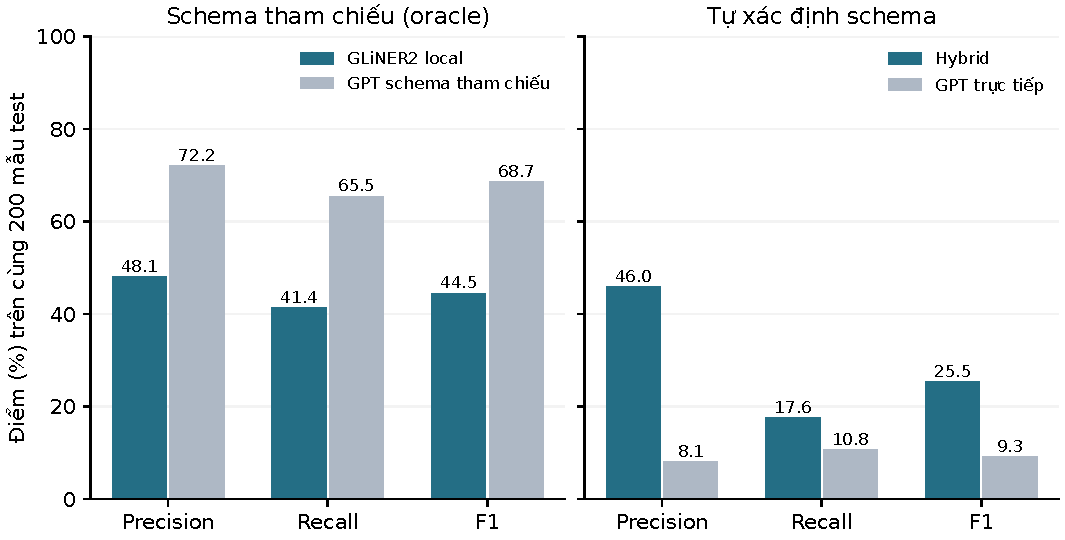
\includegraphics[width=.96\linewidth]{figures/final_comparison.pdf}
\caption{Precision, recall và fact micro F1 trên cùng 200 test, chia theo điều kiện schema tham chiếu và tự xác định schema. Hai chế độ GPT dùng kết quả đã lưu.}
\end{figure}

Cả precision và recall của hybrid đều cao hơn baseline đã lưu trong phép so sánh này. Tuy nhiên, điểm số là mức khớp của toàn bộ pipeline với gold: cách đặt tên bảng/trường, chuẩn hóa giá trị và liên kết định danh đều ảnh hưởng. Một tên gần nghĩa nhưng chưa có trong alias cố định có thể tạo FP/FN. Do đó, kết quả không đồng nghĩa GLiNER2 luôn có khả năng đọc hiểu cao hơn GPT hoặc mọi hệ thống hybrid đều sẽ tốt hơn cách tạo bảng trực tiếp.

\subsection{Độ trễ và trạng thái đầu ra của hybrid}
Hybrid có 200/200 schema hợp lệ, 187 schema chứa thuộc tính, 196 trạng thái success và bốn đầu ra trích xuất rỗng. Không có retry bên ngoài trong lượt đo. Schema không có thuộc tính vẫn có thể tạo hàng chỉ chứa định danh; vì vậy số schema có thuộc tính và số bảng rỗng không phải hai số đếm tương đương.

\begin{table}[H]
\centering
\begin{tabularx}{\linewidth}{@{}Yr@{}}
\toprule
\textbf{Chỉ số} & \textbf{Giây/bài} \\\midrule
Mean e2e & 12,020 \\
Median e2e & 11,552 \\
P95 e2e & 18,126 \\
Mean bước GPT tạo schema & 10,696 \\
Mean bước GLiNER2 & 1,310 \\
\bottomrule
\end{tabularx}

\caption{Độ trễ hybrid trên 200 mẫu; gồm GPT tạo schema và toàn bộ bước GLiNER2 cục bộ.}
\end{table}

Phần lớn độ trễ hybrid nằm ở yêu cầu GPT tạo schema; bước GLiNER2 trung bình khoảng 1,310 giây/bài. Tổng cộng GLiNER2 thực hiện 339 lượt forward để xử lý các bảng và cửa sổ văn bản cần thiết. Việc dùng mô hình cục bộ cho bước điền bảng không loại bỏ độ trễ mạng của bước tạo schema trong hybrid.

Mean 3,620 giây của GLiNER2 local và mean 12,020 giây của hybrid đều được đo trên cùng 200 mẫu test, nhưng ở hai chiến dịch và hai điều kiện schema khác nhau. Các số này mô tả độ trễ từng lượt; không tính tỷ số tăng tốc so với GPT hoặc giữa local và hybrid như một phép đo đồng thời có kiểm soát.

\subsection{Độ bao phủ schema và khác biệt giữa các bảng}
Trong 6156 dữ kiện gold của test, 2395 dữ kiện thuộc các cặp bảng--trường được schema GPT đề xuất, tương ứng 38,91\%. Có 3761 dữ kiện thuộc trường chưa được đề xuất khớp. Trong phần có trường, 1083 dữ kiện được trích khớp và 1312 dữ kiện còn chưa khớp.

\begin{figure}[H]
\centering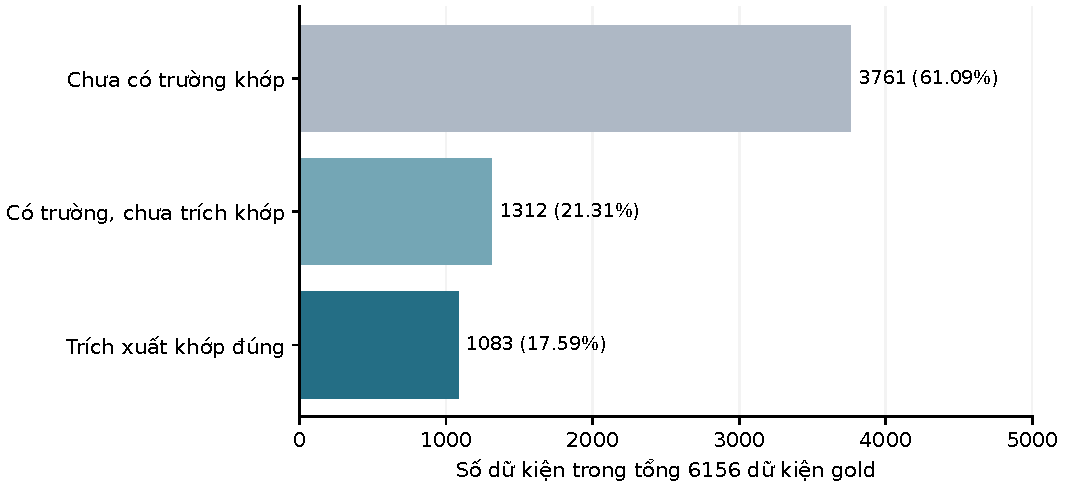
\includegraphics[width=.92\linewidth]{figures/schema_coverage.pdf}
\caption{Phân rã dữ kiện gold theo schema được đề xuất và kết quả trích xuất của hybrid.}
\end{figure}

Phân rã cho thấy hiệu quả hybrid phụ thuộc cả hai giai đoạn: chọn đúng bộ trường và điền đúng các giá trị. Tỷ lệ chưa có trường khớp cũng gồm ảnh hưởng của tên trường chưa có alias, nên không thể quy toàn bộ cho việc đoạn GPT đọc quá ngắn. Việc kiểm tra định dạng schema đạt 100\% chưa giải quyết được các vấn đề ngữ nghĩa này.

\begin{table}[H]
\centering\small\setlength{\tabcolsep}{4pt}
\begin{tabularx}{\linewidth}{@{}Yrrrrrrr@{}}
\toprule
\textbf{Bảng} & \textbf{Gold} & \textbf{TP} & \textbf{FP} & \textbf{FN} & \textbf{P (\%)} & \textbf{R (\%)} & \textbf{F1 (\%)} \\\midrule
Cầu thủ & 4839 & 1069 & 1126 & 3770 & 48,70 & 22,09 & 30,40 \\
Đội & 1317 & 14 & 106 & 1303 & 11,67 & 1,06 & 1,95 \\
\bottomrule
\end{tabularx}

\caption{Kết quả hybrid theo bảng cầu thủ và bảng đội trên 200 test.}
\end{table}

Bảng cầu thủ có 1069 dữ kiện đúng, F1 30,40\%; bảng đội chỉ có 14 dữ kiện đúng, F1 1,95\%. Điểm tổng vì vậy chưa đại diện cho chất lượng đồng đều giữa các loại bản ghi. Macro fact F1 của hybrid là 20,72\%, còn tỷ lệ tài liệu khớp hoàn toàn cả dữ kiện, trường và định danh là 0\%. Các kết quả này cho thấy vẫn cần người kiểm tra khi yêu cầu bảng đầy đủ và chính xác.

\subsection{Ý nghĩa kết quả và phạm vi áp dụng}
Kết quả local chứng minh phần trích xuất của chương trình có thể thực hiện trên CPU với thời gian đo được, phù hợp với định hướng giữ nội dung tài liệu trong môi trường nội bộ và không dùng token dịch vụ LLM cho bước này. Khi bộ trường đã được xác định rõ, đây là chế độ đáp ứng trực tiếp nhất mục tiêu xử lý hoàn toàn cục bộ.

Hybrid bổ sung khả năng đề xuất schema theo nội dung, giúp phần trích xuất không bị cố định vào một tập cột duy nhất. Trên RotoWire, cách chia vai trò này cho điểm khớp dữ kiện cao hơn GPT trực tiếp trong đối chiếu đã thực hiện. Đổi lại, đoạn văn bản dùng tạo schema vẫn được gửi tới GPT và có thể mang thông tin nội bộ; lợi ích của hybrid là giảm phạm vi dữ liệu gửi đi, không phải loại bỏ hoàn toàn việc chia sẻ dữ liệu với dịch vụ ngoài.

Khả năng dùng cho nhiều loại văn bản nằm ở cơ chế schema động và tầng trích xuất có thể tái sử dụng. Để xác nhận cho một miền mới, cần dữ liệu và nhãn của miền đó, mô tả schema phù hợp và đánh giá độc lập. Các kết quả hiện tại chỉ áp dụng cho tiếng Anh trong miền bóng rổ, một checkpoint và một mức suy luận GPT.

Ngoài ra, tập test này đã được sử dụng trong quá trình nghiên cứu trước khi đánh giá cấu hình cuối; chưa phải một tập xác nhận hoàn toàn mới. Dữ liệu cũng chưa được tách sạch theo trận và gold có thể còn thiếu hoặc sai nhãn. Vì vậy, hướng kiểm chứng tiếp theo là đánh giá trên dữ liệu chưa quan sát, tách theo sự kiện và mở rộng miền, đồng thời đo token thực nếu cần công bố mức tiết kiệm định lượng.

\subsection{Kết luận}
Dự án xây dựng phương án trích xuất bảng dựa trên GLiNER2 chạy cục bộ và mở rộng bằng GPT tạo schema từ đoạn ngắn. Trong điều kiện oracle schema tham chiếu, cấu hình local đạt F1 44,53\% trên 200 test, với độ trễ trung bình 3,620 giây/bài; GPT nhận cùng schema đạt F1 68,68\%. Hybrid đạt F1 25,46\% trên 200 test, so với 9,27\% của baseline GPT trực tiếp đã lưu, với mean e2e 12,020 giây/bài.

Giá trị của thiết kế là đưa bước đọc toàn văn và điền dữ kiện về máy cục bộ, đồng thời cho phép thay schema theo nội dung khi cần. Lợi ích về giữ dữ liệu tại chỗ đạt đầy đủ nhất ở chế độ không gọi GPT; lợi ích về giảm token dịch vụ trong hybrid mới được phân tích ở mức cơ chế, chưa được đo định lượng. Khả năng mở rộng đa miền là hướng sử dụng cần kiểm chứng thêm, còn chất lượng đầu ra hiện tại vẫn phụ thuộc độ bao phủ trường và liên kết đúng đối tượng--giá trị.

\clearpage
\addcontentsline{toc}{section}{Tài liệu tham khảo}
\begin{thebibliography}{2}
\bibitem{t2t} Xueqing Wu, Jiacheng Zhang và Hang Li (2022). \textit{Text-to-Table: A New Way of Information Extraction}. ACL, tr. 2518--2533. \url{https://aclanthology.org/2022.acl-long.180/}.
\bibitem{gliner} Urchade Zaratiana, Gil Pasternak, Oliver Boyd, George Hurn-Maloney và Ash Lewis (2025). \textit{GLiNER2: An Efficient Multi-Task Information Extraction System with Schema-Driven Interface}. EMNLP System Demonstrations, tr. 130--140. \url{https://aclanthology.org/2025.emnlp-demos.10.pdf}.
\end{thebibliography}
\end{document}
